
\subsection{Plan del proyecto}

\subsubsection{Estimación de recursos}

\begin{itemize}

  \item \textbf{ Materiales:}
	\begin{table}[H]
	 \begin{center}
	  \begin{tabular}{|l|l|c|c|}
		\hline
		\textbf{ID Unidad} & \textbf{Descripción} & \textbf{Unidad de medición} & \textbf{Nº de unidades} \\
		\hline
		HW1 & Ordenador de tipo PC & unidad & 1 \\
		\hline
		SW1 & S.O. GNU/Linux & unidad & 1 \\
		\hline
		SW2 & Intérprete de Python & unidad & 1 \\
		\hline
		SW3 & Entorno de desarrollo Eclipse & unidad & 1 \\
		\hline
	  \end{tabular}
	  \caption{Recursos materiales}
	 \end{center}
	\end{table}

  \item \textbf{Personales:}
	\begin{table}[H]
	 \begin{center}
	  \begin{tabular}{|l|l|c|c|}
		\hline
		\textbf{ID Unidad} & \textbf{Descripción} & \textbf{Unidad de medición} & \textbf{Nº de unidades} \\
		\hline
		HU1 & Análisis y diseño & horas & 130 \\
		\hline
		HU2 & Desarrollo del software & horas & 380 \\
		\hline
		HU3 & Dirección técnica & horas & 42 \\
		\hline
	  \end{tabular}
	  \caption{Recursos personales}
	 \end{center}
	\end{table}

\end{itemize}


\subsubsection{Etapas del proyecto}

El desarrollo del proyecto ha quedado delimitado en varias etapas claramente
marcadas.

Las principales etapas, también recogidas en el gráfico de gantt de la 
figura~\ref{fig:gantt}, se enumeran en la siguiente tabla:


\begin{table}[H]
 \begin{center}
  \begin{tabular}{|l|l|c|c|}
	\hline
	\textbf{WBS} & \textbf{Tarea} & \textbf{Inicio} & \textbf{Fin} \\
	\hline
	\textbf{1}   & \textbf{Especificación de requisitos y estudio de viabilidad} & 26/09/2005 & 09/01/2006 \\
	\hline
	\textbf{2}   & \textbf{Análisis y Diseño} & 09/01/2006 & 15/02/2006 \\
	\hline
	\textbf{3}   & \textbf{Desarrollo Software} & 19/01/2006 & 21/11/2006 \\
	\textbf{3.1} & Desarrollo del core de SWAML & 19/01/2006 & 18/08/2006 \\	
	\textbf{3.2} & Desarrollo de Buxon & 18/08/2006 & 01/11/2006 \\
	\textbf{3.3} & Desarrollo de herramientas complementarias & 07/09/2006 & 21/11/2006 \\	
	\hline
	\textbf{4}   & \textbf{Elaboración de la documentación} & 01/06/2006 & 30/11/2006 \\	
	\hline
	\textbf{5}   & \textbf{Dirección} & 26/09/2005 & 01/12/2006 \\
	\hline
  \end{tabular}
  \caption{Planificación de las tareas}
 \end{center}
\end{table}

\begin{figure}[p]
 	\centering
	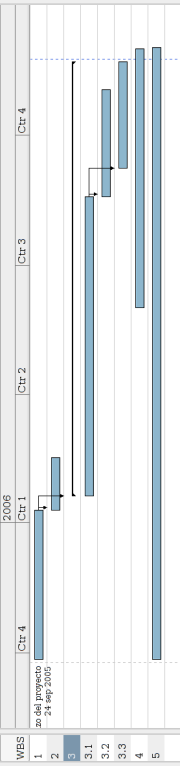
\includegraphics[width=4cm]{images/gantt.png}
	\caption{Planificación general del proyecto}
	\label{fig:gantt}
\end{figure}

\newpage

\subsubsection{Presupuesto}

\begin{itemize}

  \item \textbf{Tabla de precios:}
	\begin{table}[H]
	\begin{center}
	\begin{tabular}{|l|l|c|r|}
		\hline
		\textbf{ID Unidad} & \textbf{Descripción} & \textbf{Unidad de medición} & \textbf{Precio} \\
		\hline
		HW1 & Ordenador de tipo PC & \euro/ud & 1.190 \\
		\hline
		SW1 & S.O. GNU/Linux & \euro/ud & 0 \\
		\hline
		SW2 & Intérprete de Python & \euro/ud & 0 \\
		\hline
		SW3 & Entorno de desarrollo Eclipse & \euro/ud & 0 \\
		\hline
		HU1 & Análisis y diseño & \euro/h & 41,01 \\
		\hline
		HU2 & Desarrollo del software & \euro/h & 15,51 \\
		\hline
		HU3 & Dirección técnica & \euro/h & 59,85 \\
		\hline
	\end{tabular}
	\caption{Tabla de precios}
	\end{center}
	\end{table}

  \item \textbf{Presupuestos parciales:}
	\begin{table}[H]
	 \begin{center}
	  \begin{tabular}{|l|l|r|}
		\hline
		\textbf{ID Unidad} & \textbf{Descripción} & \textbf{Importe} \\
		\hline
		HW1 & Ordenador de tipo PC & 1.190,00 \euro \\
		\hline
		SW1 & S.O. GNU/Linux & 0,00 \euro \\
		\hline
		SW2 & Intérprete de Python & 0,00 \euro \\
		\hline
		SW3 & Entorno de desarrollo Eclipse & 0,00 \euro \\
		\hline
	  \end{tabular}
	  \caption{Presupuesto parcial de recursos materiales}
	 \end{center}
	\end{table}

	\begin{table}[H]
	 \begin{center}
	  \begin{tabular}{|l|l|r|}
		\hline
		\textbf{ID Unidad} & \textbf{Descripción} & \textbf{Importe} \\
		\hline
		HU1 & Análisis y diseño & 5.331,30 \euro \\
		\hline
		HU2 & Desarrollo del software & 5.893,80 \euro \\
		\hline
		HU3 & Dirección técnica & 2.513,70 \euro \\
		\hline
	  \end{tabular}
	  \caption{Presupuesto parcial de recursos personales}
	 \end{center}
	\end{table}	

  \item \textbf{Presupuesto final:}
	\begin{table}[H]
	 \begin{center}
	  \begin{tabular}{|l|r|}
		\hline
		\textbf{Descripción} & \textbf{Importe} \\ 
		\hline
		Recursos hardware & 1.190,00 \euro \\
		\hline
		Recursos software & 0,00 \euro \\
		\hline
		Recursos personales & 13.738,80 \euro \\
		\hline
		\textbf{SUBTOTAL} & \textbf{14.928,80 \euro} \\
		\hline
		Beneficio industrial (6\%) & 895,73 \euro \\
		\hline
		Costes generales (15\%) & 2.239,32 \euro \\
		\hline
		Suma de gastos y beneficios & 18.063,85 \euro \\
		\hline
		I.V.A. (16\%) & 2.890,22 \euro \\
		\hline
		\textbf{TOTAL} & \Large\textbf{20.954,06 \euro} \\
		\hline
	  \end{tabular}
	  \caption{Presupuesto final}
	 \end{center}
	\end{table}

\end{itemize}
